コースの幅が5つあり,それぞれの幅で十回(毎回8分間)実験する,一実験毎に,ランダムでロボットを2つグループを分ける.$T_{\rm sd}$と流量($Q$)を計測して,平均値と標準偏差を計算する.
\begin{table}[!ht]
\setlength\tabcolsep{1pt}
\begin{center}
\begin{tabular}{|c|c|c|c|c|}
\hline
幅& $\bar{T}_{\rm sd}$ & $s_{T_{\rm sd}}$ & $Q$ & $Q$ \\
($m$)   &  (分) & 標本標準偏差 & 平均値 & 標準偏差 \\
\hline
0.430 & 8.00 & 0 & 0.436 & 0.145 \\
\hline
0.495 & 6.57 & 137.346 & 3.216 & 2.814 \\
\hline
0.560 & 4.63 & 133.561 & 5.248 & 3.394 \\
\hline
0.625 & 4.57 & 106.722 & 3.29 & 2.774 \\
\hline
0.690 & 4.56 & 139.082 & 5.413 & 3.501 \\
\hline
\end{tabular}
\end{center}
\caption{
幅により$T_{\rm sd}$と流量の値
}
\end{table}
\vspace{-6mm}
\begin{figure}[!ht]
    \centering
    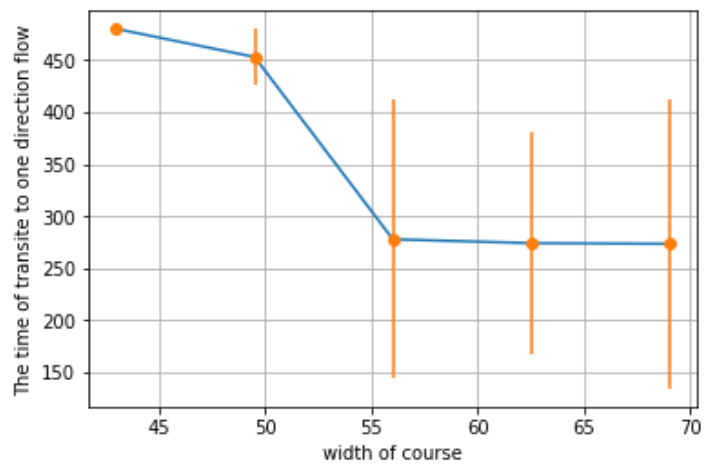
\includegraphics[width=0.8\linewidth]{diagram3.jpg}
    \caption{コース幅 $w$ と$T_{\rm sd}$の関係}
\end{figure}
\vspace{-6mm}
\begin{figure}[!ht]
    \centering
    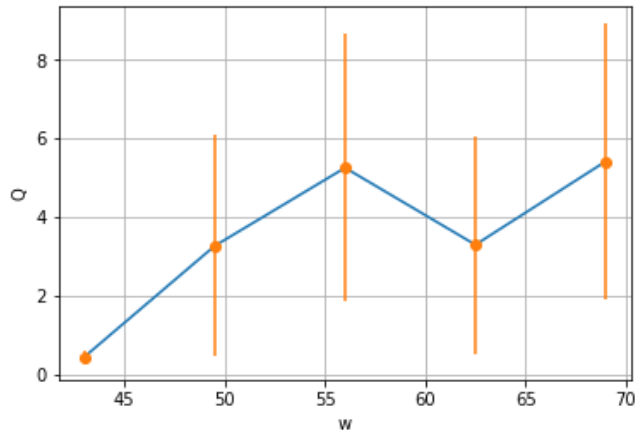
\includegraphics[width=0.8\linewidth]{diagram4.jpg}
    \caption{$Q$とコース幅の関係}
\end{figure}

図$8$はコース幅($w$)による,$T_{\rm sd}$平均値の変化曲線である.図$9$がコース幅による,平均流量($Q$)の変化曲線である.幅が狭すぎる(43$cm$)と,長時間の渋滞が発生したことを観測した,ロボット同士のすれ違い,方向転換ができず,one direction flow の状態とならなかった.大渋滞なので,流量もほとんどない.49.5$cm$の場合,渋滞が発生したので,one direction flow 状態になる時間($T_{\rm sd}$)も長かったが,ロボットが方向転換できたので,流量も多少増えた.56$cm$から渋滞の発生が急激に減少し,ロボットの方向転換もしやすくなり,$T_{\rm sd}$が減少した.以降コース幅が拡大しても,$T_{\rm sd}$に明らかな変化が見られなくなった.56$cm$まで平均流量が増えて,$62.5cm$の場合,平均流量が多少減少したと観測した.

